%%%%%%%%%%%%%
%  Ch1 : Introduction  %
%%%%%%%%%%%%%

\chapter{Introduction}
Before beginning the summary, I want to tell you that my English level isn't perfect. Please collaborate and correct the gramatically wrong sentences.\\

\section{Reminder}
	The governing equations in transport processes are the followings :
	\begin{itemize}
	\item[$\bullet$] Mass conservation : 
		\begin{equation}
			\frac{\partial \rho}{\partial t} + \nabla (\rho v) = 0
		\end{equation}
	\item[$\bullet$] Navier-Stokes :
		\begin{equation}
			\rho \left(\frac{Dv}{Dt} + v \nabla v \right) = -\nabla p + \mu \nabla ^2 v
		\end{equation}		 
	\item[$\bullet$] Energy equation :
		\begin{equation}
			\frac{DT}{Dt} = \nabla (\alpha \nabla T) + \frac{\dot{Q}v}{\rho c}
		\end{equation}
	\item[$\bullet$] Species conservation
		\begin{equation}
			\frac{\partial \rho _A}{\partial t} + \nabla (\rho _A v_A) = r_A
		\end{equation}
	\end{itemize}
	Let's precise that there are many applications using these equations like in the aerospace and automotive industry, in safety and fire prevention or in buildings design.  
	
\section{Convection and diffusion}
\subsection{Definitions}
	\begin{wrapfigure}[8]{l}{6cm}
	\vspace{-5mm}
	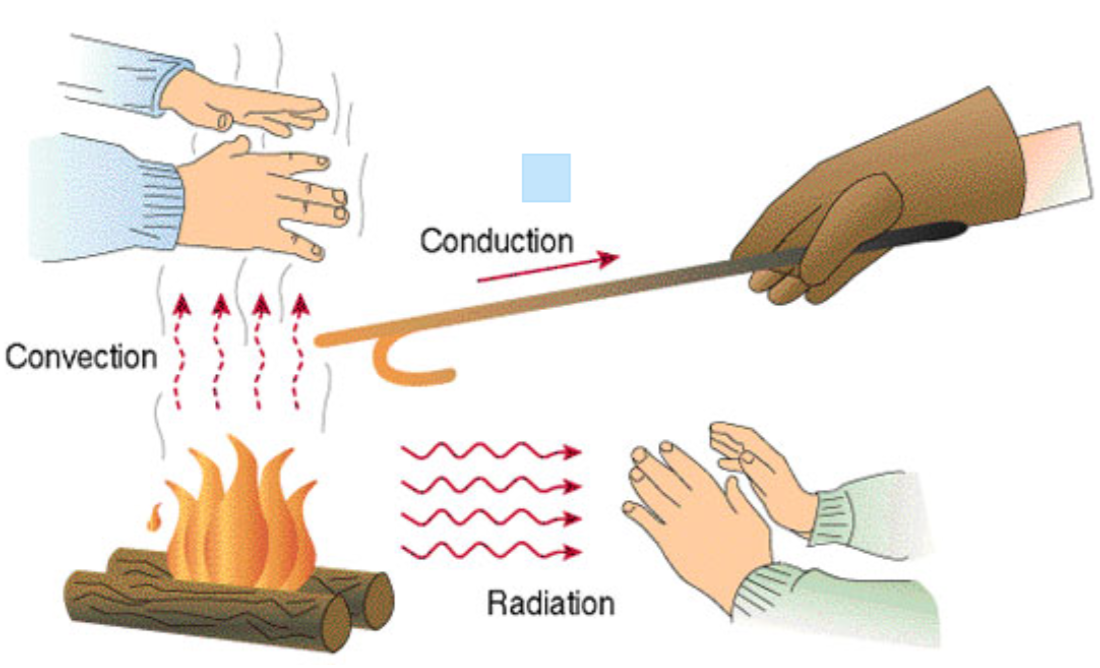
\includegraphics[scale=0.3]{ch1/1}
	\end{wrapfigure}
	Here is a picture illustrating the principles of \textbf{convection}, \textbf{conduction} and \textbf{radiation}. Imagine that you have a fire and you put your hands above. You will feel a flow of heat transmitted by convection. If someone comes with a stick, there will be conduction in the material transmitting the energy from particles to particles. Finally, if the hands are next to the fire, there is no flow but you feel the heat. The energy is transmitted by radiation. 
	
\newpage

\subsection{Convection}
	\begin{wrapfigure}[4]{r}{3.5cm}
	\vspace{-5mm}
	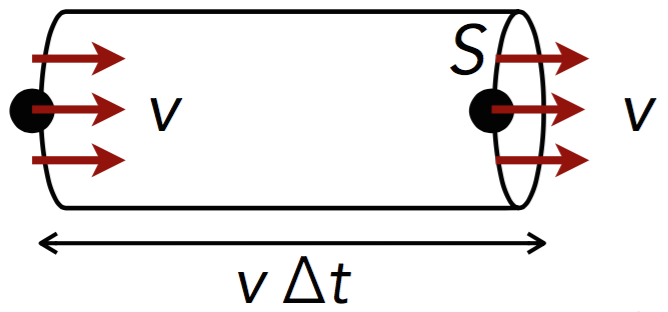
\includegraphics[scale=0.3]{ch1/2}
	\end{wrapfigure}
	Convection is a transfer always associated to \textbf{bulk (ensemble) fluid motion}. We consider a fluid with \textbf{uniform} velocity and a cylinder of section S and lenght $\Delta t$. In that time interval, the fluid in the cylinder will have crossed the section S. We are now able to express the convective flux of momentum (quantité de mouvement), energy and mass knowing that the flux of a physical quantity is given by 
	\begin{equation}
	flux _A = \frac{A}{S\Delta t}
	\label{equation:1.5}
	\end{equation}
	
\subsubsection{Mass}
	We know that the mass is given by density $\times$ volume and that the volume of the cylindre is $Sv\Delta t$. Using the new expression of the mass and \eqref{equation:1.5}, we can find the \textbf{flux of mass} 
	\begin{equation}
		M_c = \rho v S \Delta t \qquad and \qquad  J_{M_c} = \frac{M_c}{S\Delta t} = \rho v
	\end{equation}
	
\subsubsection{Momentum}
	Similarly to the calcul of the mass
	\begin{equation}
		Q_c = mv = \rho v^2 S \Delta t \qquad and \qquad J_{Q_c} = \rho v^2
	\end{equation}
	
\subsubsection{Energy}
	The energy in the system is given by the specific heat energy of each particles\footnote{See \emph{Chimie générale} for the expression}. If $T_0$ is the reference temperature, 
	\begin{equation}
		E_c = \rho c_v (T-T_0) S \Delta t \qquad and \qquad J_{E_c} = \rho c_v (T-T_0)
	\end{equation}
	
\subsection{Diffusion}
	\begin{wrapfigure}[4]{l}{3.5cm}
	\vspace{-5mm}
	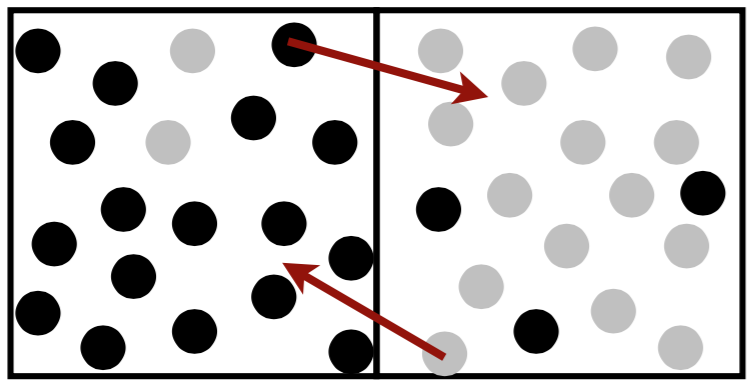
\includegraphics[scale=0.26]{ch1/3}
	\end{wrapfigure}
	Diffusion is a transfer associated to the \textbf{particles	random walk} and is due to the presence of a gradient of physical quantity (temperature for example). The picture on the left illustrates that, for an infinite time, the process will reequilibrate the gradient, difference between the two boxes.
	
\section{Diffusive flux}
	\begin{wrapfigure}[3]{r}{5.5cm}
	\vspace{-5mm}
	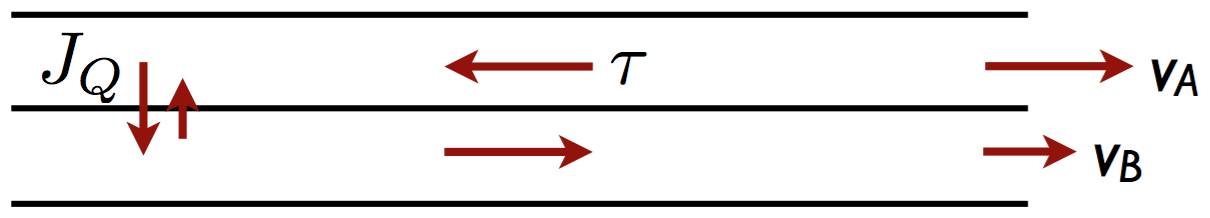
\includegraphics[scale=0.26]{ch1/4}
	\end{wrapfigure}
	If we consider two parallel fluid layers to bulk velocity $v_A > v_b$, the gradient of velocity will vanish\footnote{Disparaître} ($v_A = v_b$). This effect is due to the initial velocity gradient that cause the diffusion of faster particles towards the slower ones, transferring a momentum flux $J_Q$. In fact, the origin of the flux in the transversal direction to the flow is due to the \textbf{friction} between the two layers, parallel to the flow direction. 
	
\subsection{Shear stress}
	To characterize the friction between to layers, we introduce the \textbf{shear stress} that is proportional to the gradient of velocity
	\begin{equation}
		\tau = \tau \left( \frac{dv}{dy} \right)
	\end{equation}
	According to the Newton's law, for newtonian fluids like gases and liquids, the equation becomes
	\begin{equation}
		\tau = \mu \left( \frac{dv}{dy} \right)
	\end{equation}
	\begin{wrapfigure}[9]{l}{4cm}
%	\vspace{-5mm}
	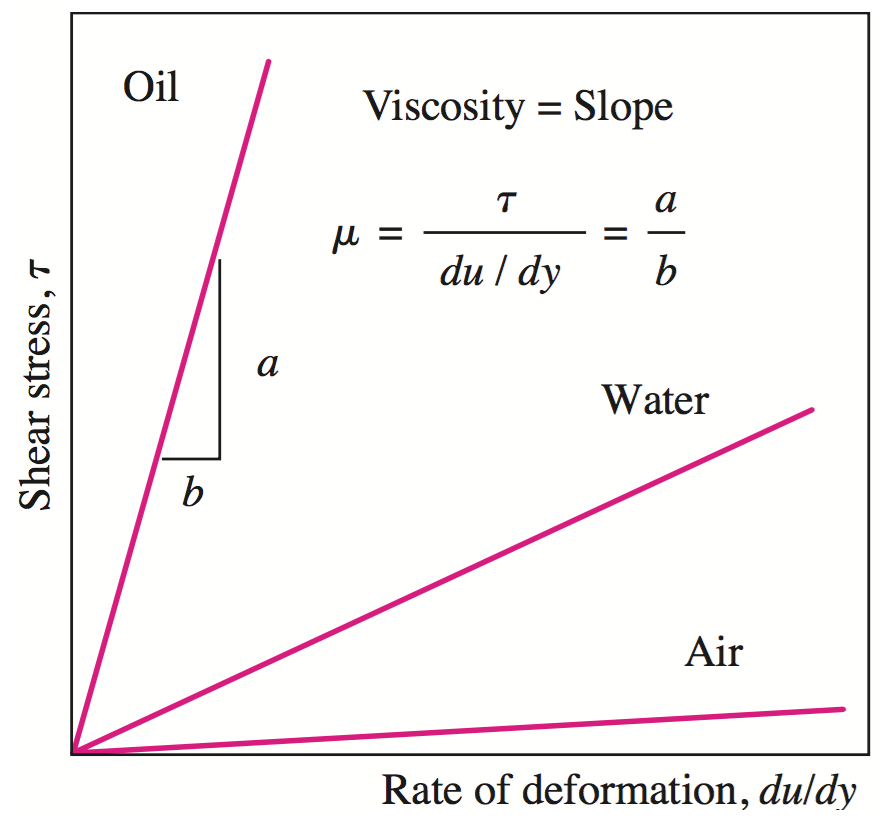
\includegraphics[scale=0.26]{ch1/5}
	\end{wrapfigure}
	\begin{itemize}
		\item $\mu$ is the \textbf{dynamic viscosity}, the \textbf{intrinsic resistance} of the fluid to motion $[kg/m.s]$
		\item $dv/dy$ the gradient of velocity $[s^{-1}]$
		\item $\tau$ a force per unit surface $[N/m^2] = [Pa]$
	\end{itemize}
	\ \\
	If we see the shear stress to the \textbf{rate of deformation} \footnote{Gradient of velocity} on a graph, we can see that the \textbf{viscosity} is the slope\footnote{La pente}. We can also see that viscosity of air is miner than water that's miner than oil. 
	
\subsection{Planar Couette flow}
	\begin{wrapfigure}[5]{r}{5.5cm}
	\vspace{-5mm}
	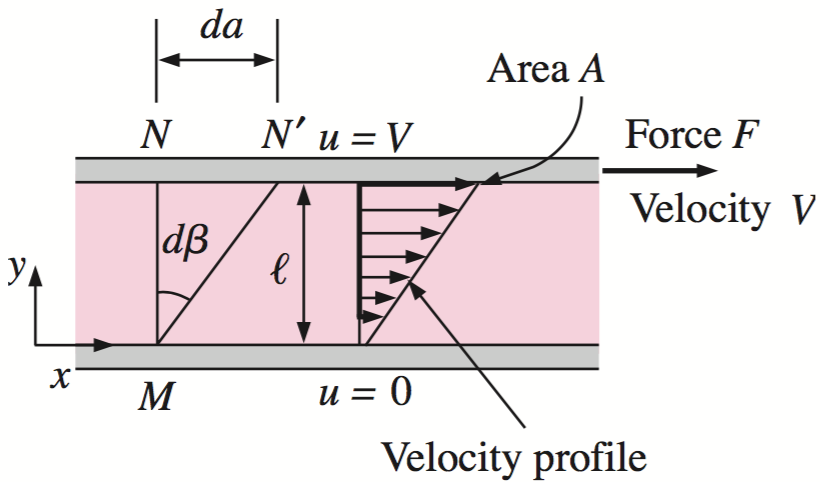
\includegraphics[scale=0.4]{ch1/6}
	\end{wrapfigure}
	Let's consider a fluid layer between two very large plates sparated by a distance $l$. A constant parallel force $F$ (drag force\footnote{Force de traînée}) is applied to the upper plate and after the initial transients, it moves continuously to a constant velocity $V$. What are the consequences on the fluid ? \\
	
	\begin{itemize}
		\item[•] \textbf{Empirical observations : }\\
		No slip conditions\footnote{Condition de non-glissement} at walls $\rightarrow u(0) = 0$ and $u(l) = V$. \\
		\item[•] \textbf{The flow is organized in parallel layers :}\\
		We suppose that the flow is laminar (no turbulence), so the velocity profile is a sole function of y and is \textbf{linear} : $u(y) = V\frac{y}{l}$.\\
		\item[•] \textbf{The drag force is imposed :} \\
			$\tau = \frac{F}{A} = \mu \frac{dv}{dy} = c$
	\end{itemize}
	
	\newpage
	
\subsection{Fluid rheology}
	\begin{wrapfigure}[12]{l}{8.5cm}
	\vspace{-5mm}
	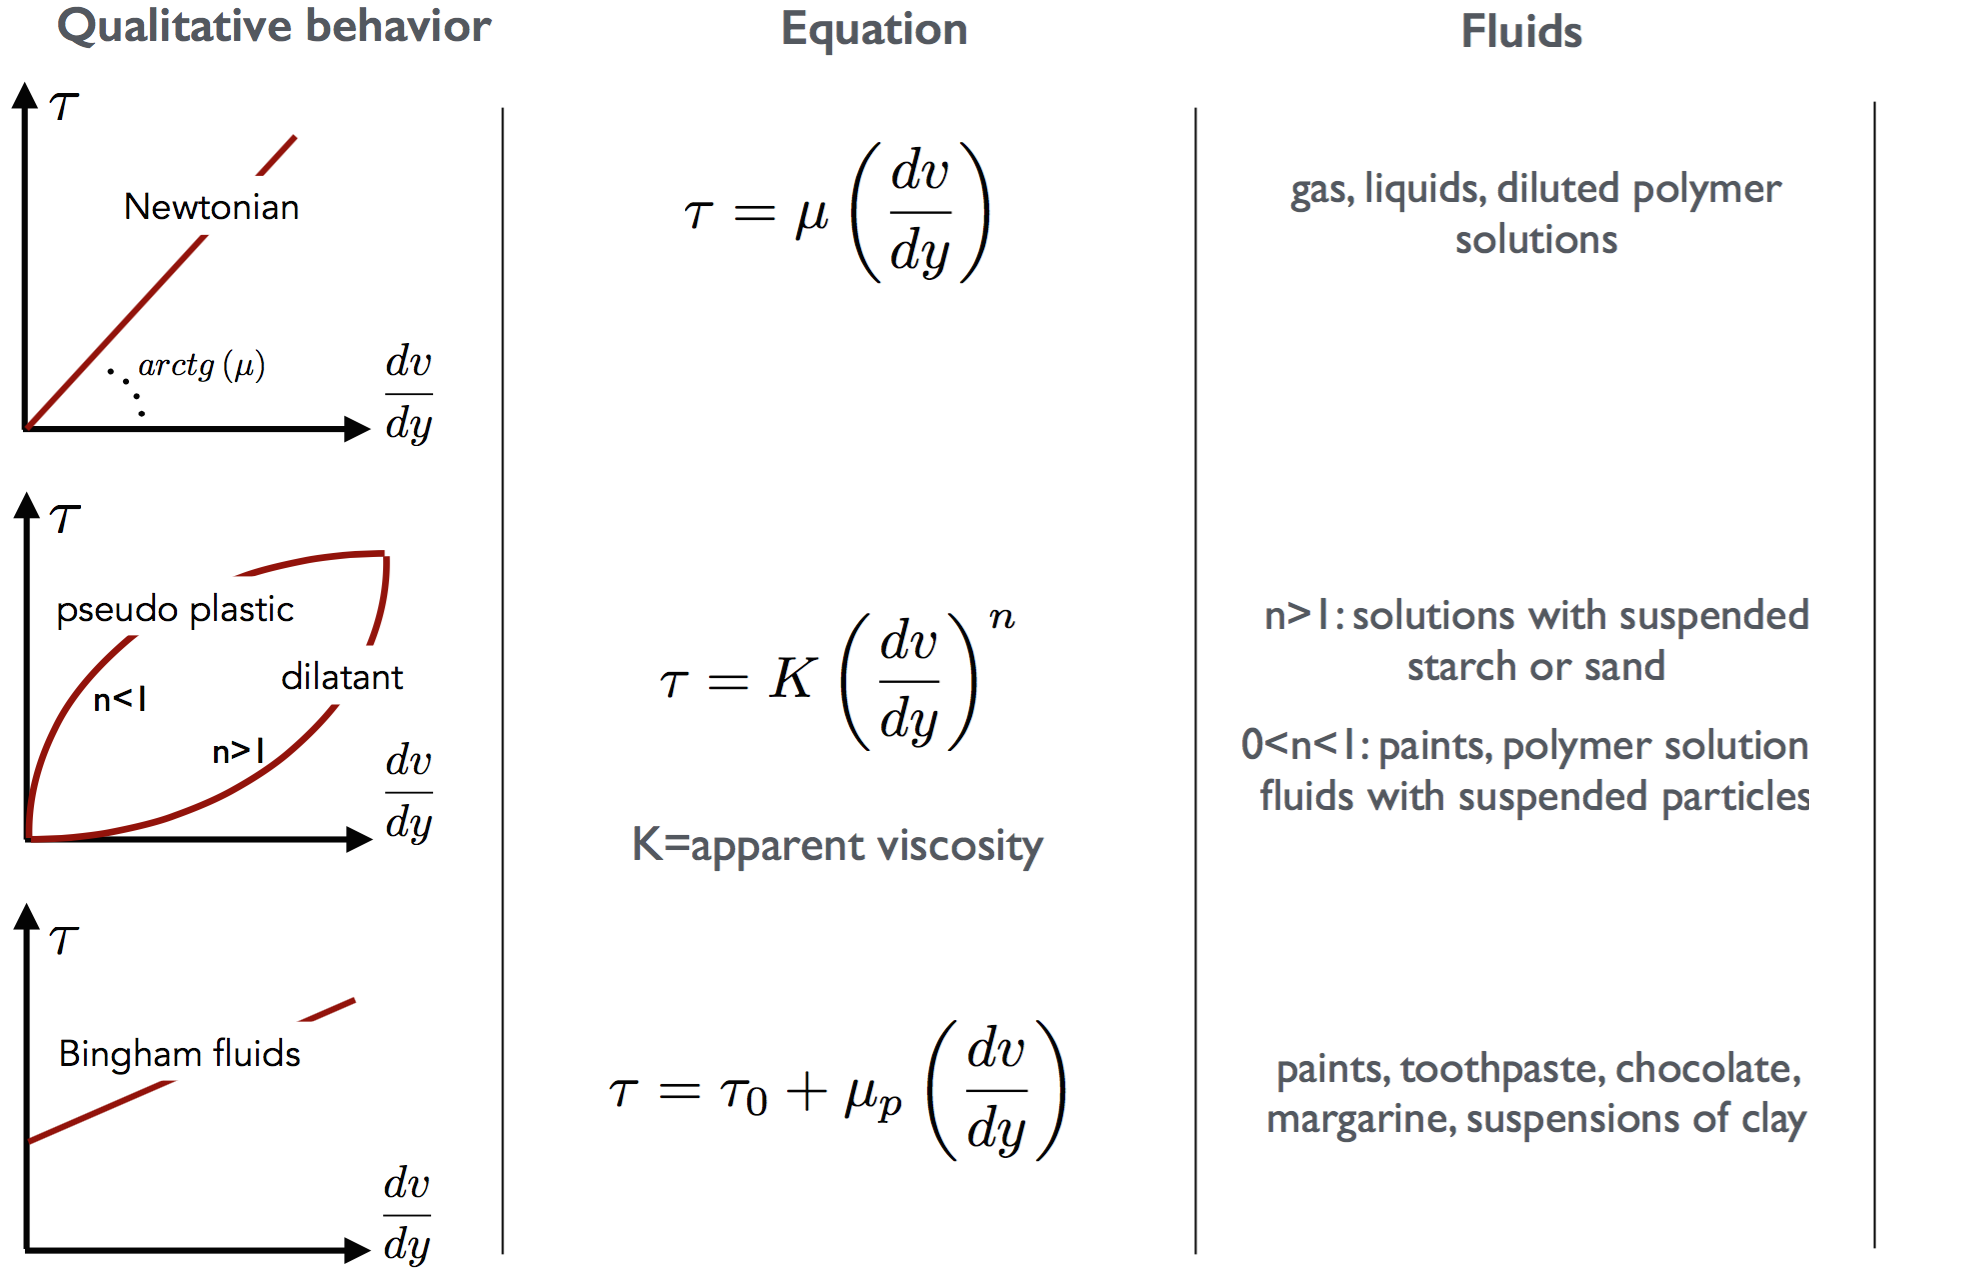
\includegraphics[scale=0.25]{ch1/7}
	\end{wrapfigure}
	\textbf{Rheology} is the study of the flow that establish the relation between the shear stress and the velocity gradient. Let's have a look to different fluids. \\
	As first observation, we can see that newtonian fluids respect a linear relation for shear stress to the rate of deformation. It's not the case for others like second and third line of the table\footnote{Starch = amidon}. For bingham fluids, there is a critical shear stress to reach before the behavior becomes like newtonian fluids 
	
\subsubsection{Dynamic viscosity of liquids and gases}	
	When we observe the table of dynamic viscosity for the water, the dynamic viscosity decreases with temperature increase for liquid water. It's not the case for the gases for wich dynamic viscosity increases with temperature. \\ The explanation is that, for liquids, the increase of temperature increases the gradient of velocity making the liquid more free. For gases, the increase of temperature makes that particles hit each other more frequently, decreasing the velocity. 
	
\section{Constitutive relations}
	It's an important section because it shows that transport processes have a uniform approach. Let's introduce 3 new variables : \textbf{kinematic viscosity} $\nu$, \textbf{thermal diffusivity }$\alpha$\textbf{internal energy} u \textbf{mass diffusivity} $D$. Let's precise that $\nu , \alpha , D = [L^2T^{-1}]$\\
	\begin{itemize}
		\item[•] \textbf{Momentum diffusion flux} (Newton's law)
		\begin{equation}
			J_{Q_d}=-\mu \frac{dv}{dy} \qquad \xrightarrow {\nu = \frac{\mu}{\rho}} \qquad J_{Q_d}=-\nu \frac{d(\rho v)}{dy}
			\label{equation:1.11}
		\end{equation}
		
		\item[•] \textbf{Energy diffusive flux} (Fourrier's law)
		\begin{equation}
			J_{E_d} = -k\frac{dT}{dy} \qquad \xrightarrow{\alpha = \frac{k}{\rho c_v} \ and \ u = c_v(T-T_0)} \qquad J_{E_d} = -\alpha\frac{d(\rho u)}{dy}
		\end{equation}
		
		\item[•] \textbf{Mass diffusion flux} (Fick's law)
		\begin{equation}
			J_{M_d} = -D \frac{dc}{dy} \qquad \mbox{($c$ = concentration)}
		\end{equation}
	\end{itemize}
	
\section{Gas viscosity}
	\begin{center}
	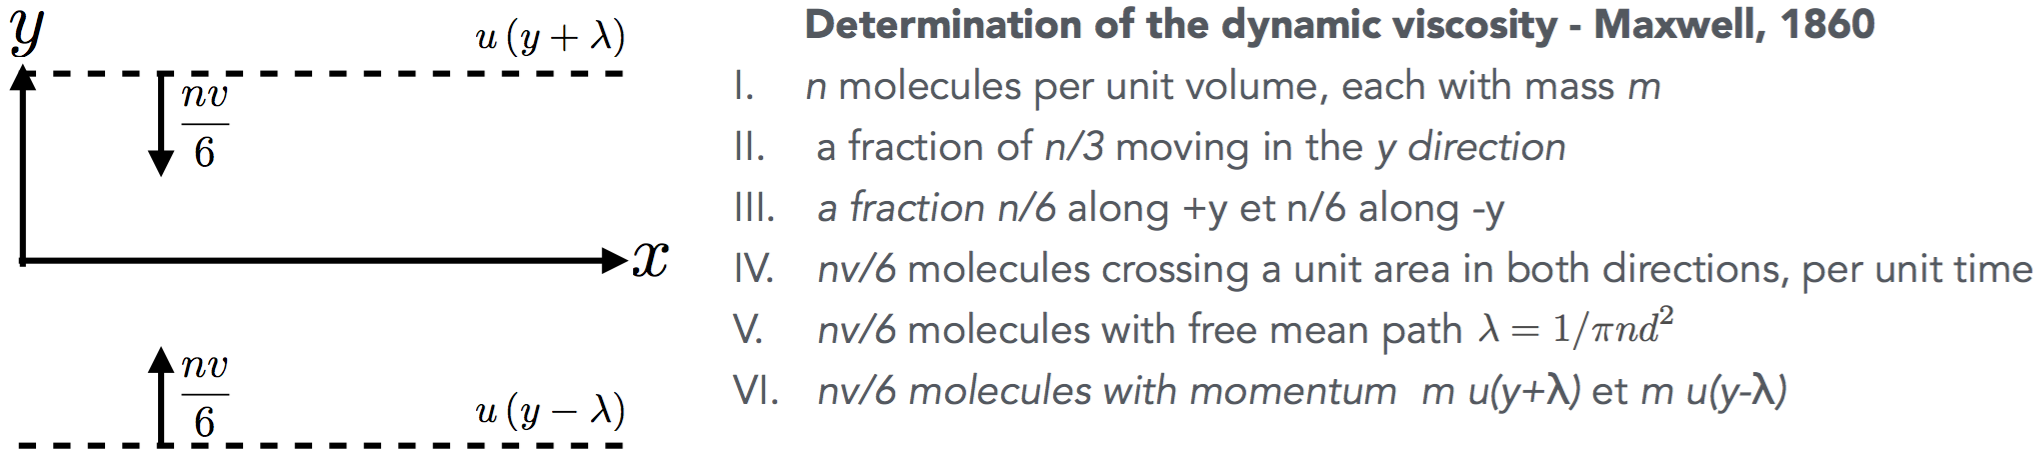
\includegraphics[scale=0.45]{ch1/8}
	\end{center}
	
	Let's consider a gas moving in the x direction with a velocity $u=u(y)$. The \textbf{kinetic theory} gives us the random velocity in $y$ using $v = \sqrt{\frac{3k_bT}{m}}$. The development of Maxwell, above, allows us to calculate the momentum flux crossing the x axis. 
	\begin{equation}
		J_{Q_d} = \left(\frac{nv}{6}\right)mu(y-\lambda) - \left(\frac{nv}{6}\right)mu(y+\lambda)
	\end{equation}
	Here we use $u(y-\lambda)$ and $u(y+\lambda)$ because the last particles that can cross an axis on y are those who are situated in a distance of maximum $\lambda$ from there. \\
	The Tylor expansion of the flux $u(y + \lambda) = u(\lambda) + \lambda\frac{du}{dy} + \dots$ and the constitutive equation \eqref{equation:1.11} gives us the final expression of viscosity 
	\begin{equation}
	\mu = \frac{1}{3}nm\lambda v = \frac{1}{3}\rho \lambda v = \frac{1}{\pi \sqrt{3}}\frac{\sqrt{mk_bT}}{d^2}
	\end{equation}